\documentclass[11pt]{article}
\usepackage{epsf}
\usepackage{hyperref}
\usepackage{graphicx}
\usepackage{subfigure}
\usepackage[margin=2.5cm]{geometry}
\usepackage{amsmath}
\usepackage{footnote}
\usepackage[bottom]{footmisc}
\usepackage[singlelinecheck=false]{caption}
\usepackage{caption}
\usepackage{amsthm}
\usepackage{enumitem}
\usepackage{graphics}
\usepackage{float}
\usepackage{amssymb}
\usepackage{natbib}
\usepackage{lscape}
\usepackage{array}
\textheight=8.7in
\usepackage{setspace}
\usepackage{verbatim}
\usepackage{multirow}
\usepackage{booktabs}
\usepackage{longtable}

\def\threedigits#1{%
  \ifnum#1<100 0\fi
  \ifnum#1<10 0\fi
  \number#1}

\topmargin=0.1in \oddsidemargin=-0.1cm \evensidemargin=-0.1cm

\paperheight=11in \paperwidth=8.5in \marginparwidth=0in

\marginparsep=0in \textwidth=6.5in \headheight=0in \headsep=0in

\onehalfspacing
\def\argmax{\mathop{\rm arg\,max}}
%\usepackage{xspace,epsfig,subfig}
\newtheorem{theorem}{Theorem}
\newtheorem{lemma}{Lemma}
\newtheorem{claim}{Claim}
\newtheorem{proposition}{Proposition}
\newtheorem{definition}{Definition}
\newtheorem{corollary}{Corollary}
\newenvironment{sketch}{\noindent\emph{Proof Sketch:}}{$\quad \Box$}
%\newenvironment{proof}{\noindent\emph{Proof:}}{$\quad \Box$}

\bibpunct{(}{)}{;}{a}{,}{,}

% operators
\DeclareMathOperator*{\argmin}{arg\,min}
\newcommand{\CV}{\operatorname{CV}}
\newcommand{\PE}{\operatorname{PE}}
\newcommand{\E}{\operatorname{E}}
\DeclareMathOperator*{\cov}{cov}
\DeclareMathOperator*{\tr}{tr}
\DeclareMathOperator*{\var}{var}

% convergence
\newcommand{\toas}{\overset{\mathit{a.s.}}{\to}}

\newcommand{\OhP}{O_p}

% sets
\newcommand{\R}{\mathbb{R}}
\newcommand{\sA}{\mathcal{A}}
\newcommand{\sbA}{\mathcal{\bar A}}
\newcommand{\sC}{\mathcal{C}}
\newcommand{\sE}{\mathcal{E}}
\newcommand{\sN}{\mathcal{N}}
\newcommand{\sX}{\mathcal{X}}

% scalars
\newcommand{\bpi}{\bar \pi}

% vectors
\newcommand{\muX}{\mu^{X}}
\newcommand{\muY}{\mu^{Y}}
\newcommand{\bmuX}{\bar \mu^{X}}
\newcommand{\bmuY}{\bar \mu^{Y}}

% matrices
\newcommand{\dataX}{\mathfrak{X}}
\newcommand{\SigmaY}{\Sigma^Y}
\newcommand{\Xtrain}{X_{\text{train}}}
\newcommand{\Ytrain}{Y_{\text{train}}}
\newcommand{\Xtest}{X_{\text{test}}}
\newcommand{\Ytest}{Y_{\text{test}}}

% class labels
\newcommand{\hGX}{\hat G^{X}}
\newcommand{\hGY}{\hat G^{Y}}


\begin{document}
\title{Estimating the number of clusters using Cross Validation}
\author{Wei Fu \qquad Patrick O. Perry \\\\ New York University}
\date{}
\maketitle
\begin{abstract}
Many clustering methods, including $k$-means, require the user to specify the
number of clusters as an input parameter. A variety of methods have been
devised to choose the number of clusters automatically, but they often rely on
strong modeling assumptions. We propose a data-driven approach to estimate the
number of clusters based on a novel form of cross-validation. This differs
from ordinary cross-validation, because clustering is fundamentally an
unsupervised learning problem. Simulation and real data analysis results show
that our proposed method outperforms existing methods, especially in
high-dimensional settings with heavy-tailed data.
\end{abstract}


\section{Introduction}

As a main task of exploratory data analysis, clustering organizes unlabeled
observations into groups such that observations in same group are more similar
compare to those in different group. Clustering is an important topic in
unsupervised learning because it can reveal the internal structure of data
through grouping, segment the data through partitioning and summarize data for
other purposes such as dimension reduction. It has being widely used in
various fields such as psychology, biology, statistics and machine learning
including pattern recognition, image segmentation etc.


After being proposed more than $50$ years, $k$-means remains one of the most
popular and widely used clustering algorithms \citep{jain2010data}. Like many
other clustering methods, $k$-means requires an input parameter $k$, the
number of clusters, to be specified by the user. Automatically and
quantitatively deciding such parameter is important and yet unsolved problem
\citep{fujita2014non}. Various methods have been proposed to tackle this
difficulty. One ad hoc approach is to explore the relationship between $W_k$
(within-cluster dispersion) and the number of cluster $k$ for a certain
clustering method such as $k$-means. Since $W_k$ decreases as $k$ increases,
one usually find the ``elbow" of curve obtain by plotting $W_k$ versus $k$ as
the appropriate number of clusters. The example on the top row of
Figure~\ref{fig:elbow} demonstrates such approach for data with $k=4$, where
the ``elbow" point indeed reveals the true number of clusters. This is based
on the idea that under partitioning data set has more impact than over
partitioning data set in terms of $W_k$. However, locating the ``elbow" point
is somewhat subjective and sometimes is not appropriate to select the optimal
$k$. The second example on the bottom row of Figure \ref{fig:elbow} shows a
situation where there is no clear choice of the ``elbow" point -- both $k=2$
and $k=3$ can be viewed as the ``elbow" point. What's more, the true $k=4$ can
never be selected as the optimal $k$ using such approach in this case since it
can hardly be viewed as the ``elbow" of the curve.


\begin{figure}
\centering
\begin{minipage}{\linewidth}
  \begin{minipage}{0.45\linewidth}
    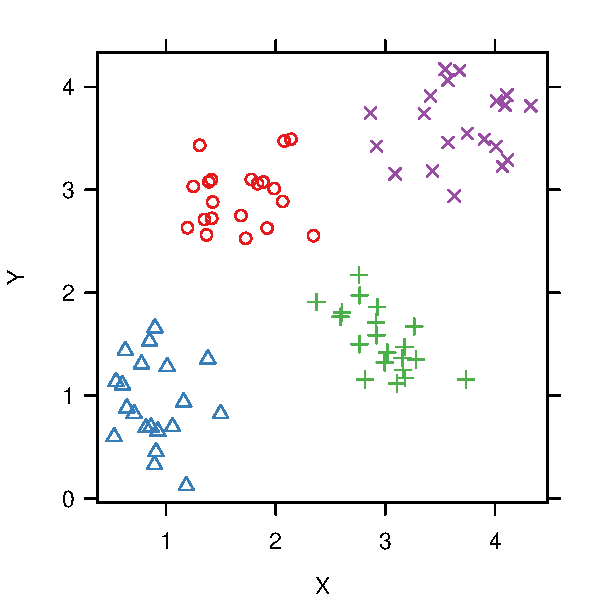
\includegraphics[width=\linewidth]{demo/elbow/correct-data.pdf}
  \end{minipage}
  \hspace{0.05in}
  \begin{minipage}{0.45\linewidth}
    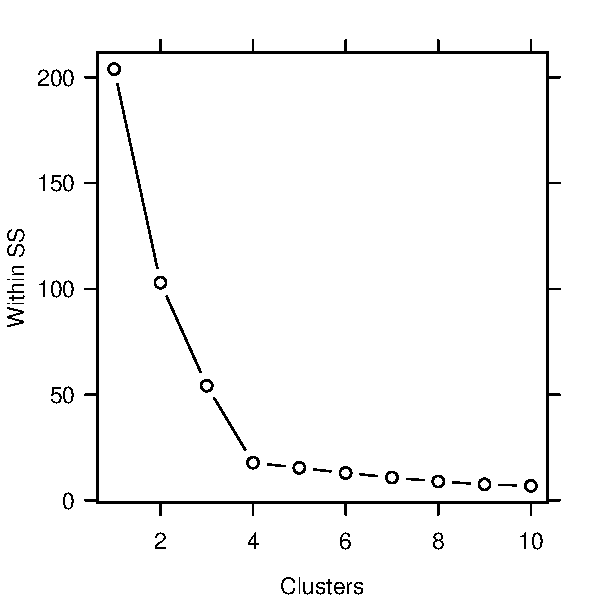
\includegraphics[width=\linewidth]{demo/elbow/correct-withinss.pdf}
  \end{minipage}
\end{minipage}
\begin{minipage}{\linewidth}
  \begin{minipage}{0.45\linewidth}
    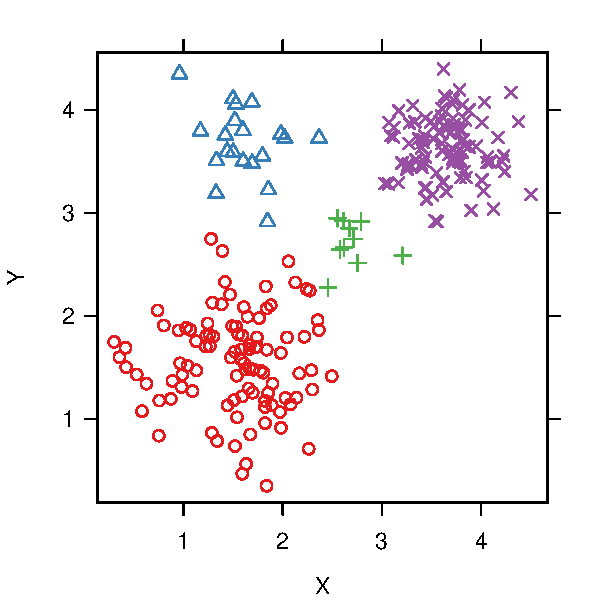
\includegraphics[width=\linewidth]{demo/elbow/incorrect-data.pdf}
  \end{minipage}
  \hspace{0.05in}
  \begin{minipage}{0.45\linewidth}
    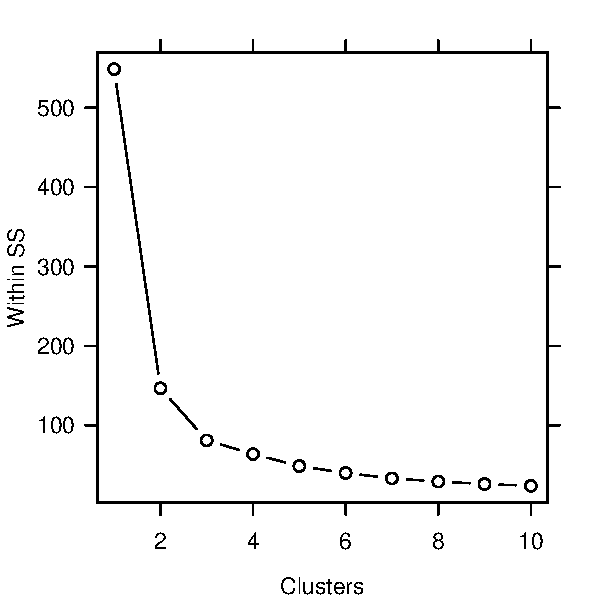
\includegraphics[width=\linewidth]{demo/elbow/incorrect-withinss.pdf}
  \end{minipage}
\end{minipage}
\caption{Left panels show the $(X,Y)$ data points; right panels
  show the corresponding values of the within-cluster sum of squares $W_k$
plotted against the number of clusters, $k$.}
\label{fig:elbow}
\end{figure}


Recently, there are several new proposals to find the $k$ automatically. Gap
statistics \citep{tibshirani2001estimating} estimates $k$ by comparing the
change in within-cluster dispersion with that expected under an appropriate
reference null distribution. Specifically, the graph of $\log(W_k)$ is
compared with its expectation under an appropriate null reference distribution
of the data. The value of $k$ associated with the largest gap between
$\log(W_k)$ and the reference curve is selected as optimal $k$.
\citet{sugar2003finding} proposed an approach which finds the number of
clusters based on distortion, a quantity that measures the average distance,
per dimension. It's backed by a rigorous theoretical justification based on
information-theoretic ideas.   \citet{fraley2002model}'s Model-based method
employs the EM algorithm to estimate the parameters in Gaussian mixture model,
and select the best model ($k$) using BIC criterion. Stability-based criterion
is also proposed to locate the best $k$ by some authors such as
\citet{ben2001stability}, \citet{wang2010consistent} and
\citet{fang2012selection}. \citet{chiang2010intelligent} provides a nice review
of existing methods for finding the right $k$ in published literature.


Most existing methods are either model based method requires strong parameter
assumptions or ad hoc method utilizes within-cluster dispersion. Although many
view selecting the number of clusters as a model selection problem, very few
approaches this problem from the prediction point of view. Select model with
smallest prediction error via cross-validation is one of the simplest and most
widely used model selection techniques in supervised learning. The lack of
true class (label) in data set makes the adoption of cross-validation into
unsupervised leaning problem difficult. Perhaps the only exception is
\cite{tibshirani2005cluster}, which selects the optimal $k$ by prediction
strength. The strategy is to first cluster the test data and training data
into $k$ clusters respectively. Then, for each pair of observations that are
assigned to the same test cluster, algorithm determines whether they are also
assigned to the same cluster based on the training centers. The intuition here
is, if $k=k_0$, the true number of clusters, then the $k$ training set
clusters will be similar to the $k$ test clusters, and hence will predict them
well. However, a specifically defined prediction error measure is used in such
procedure, which is quite different from the one commonly used in
cross-validation procedure in supervised learning. Therefore the well
understood properties of cross-validation procedure in supervised learning
cannot be carried over to the prediction strength method, makes the
interpretation of its result difficult.


Our proposed method is a complete data-driven approach which doesn't rely on
any parametric assumptions. Through novel form of partitioning data set, we
are able to employing the cross-validation procedure in clustering exactly the
same way as in supervised learning problem. Hence, it's easy for reader to
understand the intuition behind our proposed method. Simulation and real data
application shows the superior performance of our proposed method compare with
existing methods in high-dimension settings and heavy-tailed data. Since the
embedded cross-validation procedure is well understood, it also makes our
method potentially easily to be extended in future study. 
 


\section{Cross-validation for selecting the number of clusters}

Cross-validation is commonly used for model selection in supervised learning
problems.  In these settings, the data comes in the form of $N$
predictor-response pairs, $(X_1, Y_1), \dotsc, (X_N, Y_N)$, with $X_i \in
\R^{p}$ and $Y_i \in \R^{q}$.  The data can be represented as a matrix with
$N$ rows and $p + q$ columns.  We partition the data into $K$ hold-out
``test'' subsets, with $K$ typically chosen to be $5$ or $10$.  For each
``fold'' $r$ in the range $1, \dotsc, K$, we permute the rows of the data
matrix to get $\dataX$, a matrix with the $r$th test subset as its trailing
rows.  We partition $\dataX$ as
\[
  \dataX =
  \begin{bmatrix}
    \Xtrain & \Ytrain \\
    \Xtest  & \Ytest
  \end{bmatrix}.
\]
We use the training rows $[ \Xtrain\ \Ytrain ]$ to fit a regression model
$\hat Y = \hat Y(X)$, and then evaluate the performance of this model on the
test set, computing the cross-validation error $\|\Ytest - \hat Y(\Xtest)\|^2$
or some variant thereof.  We choose the model with the smallest
cross-validation error, averaged over all $K$ folds.


In unsupervised learning problems like factor analysis and clustering, the
features of the observations are not naturally partitioned into ``predictors''
and ``responses'', so we cannot directly apply the cross-validation procedure
described above.  For factor analysis, there are at least two versions of
cross-validation.  \citet{wold78cross} proposed a ``speckled'' holdout, where
in each fold we leave out a subset of the elements of the data matrix.  Wold's
procedure works well empirically, but does not have any theoretical support,
and it requires a factor analysis procedure that can handle missing data.
\citet{owen2009bi} proposed a scheme called ``bi-cross-validation'' wherein
each fold designates a subset of the data matrix columns to be response and a
subset of the rows to be test data.  This generalized a procedure due to
\citet{gabriel2002biblot}, who proposed holding out a single column and a
single row at each fold.  Owen and Perry proved that this procedure is
self-consistent, in the sense that it performs the correct model selection in
the absence of noise, and \citet{perry2009cross} provided more theoretical
support.


In this report, we extend the Wold and Gabriel methods to the clustering
problem, specifically to choose an appropriate number of clusters for a
dataset.  We prove that the Gabriel method is self-consistent, and we analyze
some of its properties in the presence of noise.  We compare these methods to
state-of-the-art algorithms, and show that both are competitive.



%% [POP] This paragraph doesn't fit into the section.  Maybe put it in the introduction?
%% 
%% Cross-Validation technique, one of the most commonly used and popular model
%% selecting method in supervised learning, can not be used naively in
%% unsupervised learning context. Since prediction error of new observation is
%% calculated by its distance to the nearest cluster center, more cluster centers
%% means much tighter fit to the feature space, and hence smaller distance
%% (prediction error) of observation to its nearest cluster center. This holds
%% even when the prediction is evaluated on an independent test set
%% \citep{hastie2009elements}. Therefore, CV prefers larger $k$ if we do the CV
%% naively.




We now give the details of how to implement
the Gabriel cross-validation to locate the optimal cluster number $k$. The
Wold cross-validation algorithm is described in Appendix $A$.


\subsection{Gabriel CV algorithm}
\label{sec:gabriel-cv-algorithm}

We are given a data matrix with $N$ rows and $P$ columns.  In each fold of
cross-validation, we permute the rows and columns of the data matrix and then
partition the rows and columns as $N = n + m$ and $P = p + q$ for 
non-negative integers $n$, $m$, $p$, and $q$.  We treat the first $p$
columns as ``predictors'' and the last $q$ columns as ``responses'';
similarly, we treat the first $n$ rows as ``training'' and the last $m$ rows
as ``test''.  In block form, the permuted data matrix is
\[
  \dataX
  =
  \begin{bmatrix}
    \Xtrain & \Ytrain \\
    \Xtest  & \Ytest
  \end{bmatrix},
\]
where
$\Xtrain \in \R^{n \times p}$,
$\Ytrain \in \R^{n \times q}$,
$\Xtest \in  \R^{m \times p}$,
and
$\Ytest \in  \R^{m \times q}$.


Given such a partition of $\dataX$, we perform four steps for each value of
$k$, the number of clusters:
\begin{enumerate}
  \item \label{step:gabriel-cluster}
    \textbf{Cluster:}
    Cluster $Y_{1}, \dotsc, Y_n$, the rows of $\Ytrain$, yielding the
    assignment rule $\hGY : \R^q \to \{ 1, \dotsc, k \}$ and the
    cluster means $\bmuY_1, \dotsc, \bmuY_k$.  Set $\hGY_i = \hGY(Y_i)$ to
    be the assigned cluster for row $i$.

  \item \label{step:gabriel-classify}
    \textbf{Classify:}
    Take $X_{1}, \dotsc, X_n$, the rows of $\Xtrain$ to be predictors,
    and take $\hGY_1, \dotsc, \hGY_n$ to be corresponding class labels.  Use
    the pairs $\{ (X_i, \hGY_i) \}_{i=1}^{n}$ to train a classifier
    $\hGX : \R^p \to \{ 1, \dotsc, k \}$.

  \item \label{step:gabriel-predict}
    \textbf{Predict:}
    Apply the classifier to $X_{n+1}, \dotsc, X_{n+m}$, the rows of
    $\Xtest$, yielding predicted classes $\hGX_i = \hGX(X_i)$ for
    $i = n+1, \dotsc, n+m$.  For each value of $i$ in this range, compute
    predicted response $\hat Y_i = \bmuY(\hGX_i)$, where
    $\bmuY(g) = \bmuY_g$.

  \item \label{step:gabriel-evaluate}
    \textbf{Evaluate:}
    Compute the cross-validation error
    \[
      \CV(k) = \frac{1}{m} \sum_{i=n+1}^{n+m} \|Y_i - \hat Y_i\|^2,
    \]
    where $Y_{n+1}, \dotsc, Y_{n+m}$ are the rows of $\Ytest$.
\end{enumerate}
\noindent
In principle, we could use any clustering and classification methods in
steps~\ref{step:gabriel-cluster} and~\ref{step:gabriel-classify}.  In this
report, we use $k$-means as the clustering algorithm.  For the classification
step, we compute the mean value of $X$ for each class; we assign an
observation to class $g$ if that class has the closest mean (randomly breaking
ties between classes).  The classification step is equivalent to linear
discriminant analysis with equal class priors and identity noise covariance
matrix.


To choose the folds, we randomly partition the rows and columns into $K$ and
$L$ subsets, respectively.  Each fold is indexed by a pair $(r,s)$ of
integers, with $r \in \{1, \dotsc, K\}$ and $s \in \{1, \dotsc, L\}$.  Fold
$(r,s)$ treats the $r$th row subset as ``test'', and the $s$th column subset
as ``response''.  We typically take $K = 5$ and $L = 2$.  For the number of
clusters, we select the value of $k$ that minimizes the average of $\CV(k)$
over all $K \times L$ folds (choosing the smallest value of $k$ in the event
of a tie).



\section{Self-Consistency of Gabriel CV method}


This section gives the self-consistency proof of the proposed Gabriel method.
Specifically, we will show that under appropriate conditions, in the absence
of noise, the Gabriel cross-validation procedure finds the optimal number of
clusters.


Because $k$-means algorithm is essential to the method, we review the
procedure here.  Given a set of observations $\{ x_1, \dotsc ,x_n \}$, and a
specified the number of clusters $k$, the goal of the $k$-means procedure is
to find a set of $k$ or cluster centers $A = \{ a_1, \dotsc, a_k \} $
minimizing the within cluster dispersion
\[
  W(A) = \sum_{i=1}^{n} \min_{a \in A} \|x_i - a\|^2.
\]
This implicitly defines a cluster assignment rule
\[
  g(x) = \argmin_{g \in \{1, \dotsc, k\}} \|x - a_g\|^2,
\]
with ties broken arbitrarily.  We will assume that the $k$-means procedure
finds an optimal solution, $A$, but we will not assume that this solution is
unique.


It will suffice to analyze a single fold of the cross-validation procedure.
As in in section~\ref{sec:gabriel-cv-algorithm} we assume that the $P$
variables of the data set have been partitioned into $p$ predictor variables
represented in vector~$X$ and $q$ response variables represented in
vector~$Y$.  The $N$ observations have been divided into two sets: $n$ train
observations and $m$ test observations.  The following theorem gives
conditions for Gabriel CV to recover the true number of clusters in the
absence of noise.


\begin{theorem}\label{thm:self-consistency}

Let $\{ (X_i, Y_i) \}_{i=1}^{n+m}$ be the data from a single fold of Gabriel
cross-validation.  For any $k$, let $CV(k)$ be the cross-validation error for
this fold, computed as described in Section~\ref{sec:gabriel-cv-algorithm}.
We will assume that there are $K$ true centers $\mu(1), \dotsc,\mu(K)$, with
the $g$th cluster center partitioned as $\mu(g) = \bigl(\muX(g),
\muY(g)\bigr)$ for $g = 1, \dotsc, K$.  Suppose that
\begin{enumerate}[label=(\roman*)]
  \item \label{asn:self-consistency-noiseless}
    Each observation $i$ has a true cluster $G_i \in \{ 1, \dotsc, K \}$.
    There is no noise, so that $X_i = \muX({G_i})$ and $Y_i = \muY(G_i)$ for
    $i = 1, \dotsc, n+m$.

  \item \label{asn:self-consistency-distinct-mux}
    The vectors $\muX(1), \dotsc,\muX(K)$ are all distinct.

  \item \label{asn:self-consistency-distinct-muy}
    The vectors $\muY(1), \dotsc,\muY(K)$ are all distinct.

  \item \label{asn:self-consistency-train}
    The training set contains at least one member of each cluster: for all $g$
    in the range $1, \dotsc, K$, there exists at least one $i$ in the range
    $1, \dotsc, n$ such that $G_i = g$.

  \item \label{asn:self-consistency-test}
    The test set contains at least one member of each cluster: for all $g$ in
    the range $1, \dotsc, K$, there exists at least one $i$ in the range $n+1,
    \dotsc, n+m$ such that $G_i = g$.

\end{enumerate}
Then $CV(k) < CV(K)$ for $k < K$, and $CV(k) = CV(K)$ for $k > K$, so that
Gabriel CV correctly chooses $k = K$.
\end{theorem}

This theorem is implied by the following two lemmas.

\begin{lemma}
Suppose that the assumptions of Theorem~\ref{thm:self-consistency} are in
force.  If $k < K$, then $\CV(k) > 0$.
\end{lemma}
\begin{proof}
By definition,
\[
  \CV(k)
    =
      \sum_{i=n+1}^{n+m}
        \| Y_i - \bmuY (\hGX_i) \|^2,
\]
where $\bmuY(g)$ is the center of cluster $g$ returned from applying $k$-means
to $Y_1, \dotsc, Y_n$.  Assumptions~\ref{asn:self-consistency-noiseless}
and~\ref{asn:self-consistency-test}, imply that as $i$ ranges over the test
set $n+1, \dotsc, n+m$, the response $Y_i$ ranges over all distinct values in
$\{ \muY(1), \dotsc, \muY(K) \}$.
Assumption~\ref{asn:self-consistency-distinct-muy} implies that there are
exactly $K$ such distinct values.  However, there are only $k$ distinct values
of $\bmuY(g)$.  Thus, at least one summand
\(
  \| Y_i - \bmuY(\hGX_i) \|^2
\)
is nonzero.  Therefore,
\(
  \CV(k) > 0.
\)
\end{proof}


\begin{lemma}
Suppose that the assumptions of Theorem~\ref{thm:self-consistency} are in
force.  If $k \geq K$, then $\CV(k) = 0$.
\end{lemma}
\begin{proof}
From assumptions~\ref{asn:self-consistency-noiseless},
\ref{asn:self-consistency-distinct-muy},
and~\ref{asn:self-consistency-train}, we know the cluster centers
gotten from applying $k$-means to $Y_1, \dotsc, Y_n$ must include
$\muY(1), \dotsc, \muY(K)$.  Without loss of generality, suppose that
$\bmuY(g) = \muY(g)$ for $g = 1, \dotsc, K$.  This implies that
$\hGY_i = G_i$ for $i = 1, \dotsc, n$.  Thus, employing
assumption~\ref{asn:self-consistency-noiseless} again, we get that
$\bmuX(g) = \muX(g)$ for $g = 1, \dotsc, K$.


Since assumption~\ref{asn:self-consistency-distinct-mux} ensures that
$\muX(1), \dotsc, \muX(K)$ are all distinct, we must have that $\hGX_i = G_i$
for all $i = 1, \dotsc, m+n$.  In particular, this implies that $\bmuY(\hGX_i)
= Y_i$ for $i = 1, \dotsc, m+n$, so that $\CV(k) = 0$.
\end{proof}

The following lemma is not required for the $k$-means consistency theorem, but
it will prove necessary for analyzing the asymptotic behavior of Gabriel
cross-validation.


\begin{lemma}\label{lem:kmeans-separation}
Set $\mu = \int x P(dx)$.  If $\int \|x\|^2 P(dx) < \infty$, then there exists
an $r > 0$ such that for every $A \in \sbA_k$, there is at most one center $a
\in A$ with $\|a - \mu\| \leq r$.
\end{lemma}
\begin{proof}
If the support of $P$ has fewer than $k$ points, then the result is trivial.
Otherwise, Lemma~\ref{lem:kmeans-existence} implies that $m_k(P) <
m_{k-1}(P)$.  Define
\[
  d =
    \inf_{A \in \sA_k}
      \min \{ \|a - a'\| : a,a' \in A, a \neq a' \}.
\]
If $d = 0$, then there exists a sequence $A_n$ in $\sbA_k$ with
\[
  \min_{\substack{a,a' \in A_n \\ a \neq a'}} \|a - a'\| \to 0.
\]
Since $\sbA_k$ is compact, there exists a subsequence $n(m)$ and a set $A_0
\in \sbA_k$ with $A_{n(m)} \to A_0$.  Take $B_n \in \sA_{k-1}$ to be the set
formed by removing one of the centers $a'$ minimizing $\min_{\substack{a \in
A_n \\ a \neq a'}} \|a - a'\|$.  By construction, $H(A_n, B_n) \to 0$, so that
$B_{n(m)} \to A_0$.  Since the map $A \mapsto W(A, P)$ is continuous on
$\sA_k$, we must have $W(B_{n(m)}, P) \to W(A_0, P) = m_k(P)$.  However, this
is impossible since $W(B_n,P) \geq m_{k-1}(P) > m_k(P)$.  It must be the case,
then, that $d > 0$.


Set $r < d/2$, and let $A \in \sbA_k$ be arbitrary.  Take $a_1$ to be the
cluster center in $A$ closest to $\mu$ (breaking ties arbitrarily).  If $\|a_1
- \mu\| > r$, then $\|a - \mu\| > r$ for all centers $a \in A$.  Otherwise, if
$\|a_1 - \mu\| \leq r$ and $a \in A$ is any other cluster center, then
\(
  2r < \|a - a_1\| \leq \|a - \mu\| + \|a_1 - \mu\|
\)
so that
\(
  \|a - \mu\| > r.
\)
\end{proof}



\section{Analysis of Gabriel Cross-Validation with Gaussian Noise}

\subsection{Single Cluster}

Now we we analyze the asymptotic performance of Gabriel Cross-Validation, in
the case of Gaussian noise. Our main result is that with single-cluster
Gaussian data, if the predictor and response columns of $\dataX$ are weakly
correlated or independent, then the method will correctly prefer $k = 1$ to
$k = 2$ clusters. We state the result in the case where $\dataX$ has 2 columns,
but it is straightforward to generalize this result to higher dimensions.

\begin{proposition}
Suppose that $\{ (X_i, Y_i) \}_{i=1}^{n + m}$ is data from a single fold
of Gabriel cross-validation, where each $(X,Y)$ pair in $\R^2$ is an
independent draw from a mean-zero multivariate normal distribution with unit
marginal variances and correlation $\rho$.  In this case, the data are drawn
from a single cluster; the true number of clusters is~$1$.  If $|\rho| < 0.5$,
then $\CV(1) < \CV(2)$ with probability tending to one as $m$ and $n$ increase.
\end{proposition}

\begin{proof}

Given $(X_1, Y_1), \dotsc, (X_n, Y_n)$, we first apply $k$-means to $\{ Y_i
\}_{i=1}^{n}$. With $k = 1$, the single-cluster centroid will
be equal to $\bar Y_n$, the sample mean of the $Y_1, \dotsc, Y_n$, approximately equal to
$\E(Y) = 0$, with error of size $\OhP(n^{-1/2})$. The cross-validation error
will be
\[
  \CV(1) = \frac{1}{m} \sum_{i=n+1}^{n+m} \| Y_i - \bar Y_n \|^2
         = 1 + \OhP(m^{-1/2}) + \OhP(n^{-1/2}).
\]

Now we will consider the $k = 2$ case.  If $n$ is large enough, then
\citet{pollard1981strong} showed that the centroids $\bmuY_1$ and $\bmuY_2$
will be close to $\E(Y \mid Y > 0) = \sqrt{2/\pi}$ and $\E(Y \mid Y < 0) =
-\sqrt{2/\pi}$.  We have used Lemma~\ref{lem:truncated-normal-moments}
(Appendix~\ref{app:technical-lemmas}) to compute the expectations.  Further,
\citet{pollard1982central} showed that the errors will be of size $\OhP(n^{-1/2})$.


If $\rho > 0$ and $n$ is large enough, then classification rule learned from
$\{(X_i, \hGY_i)\}_{i=1}^{n}$ variables will be determined according to
whether $X > 0$; if $\rho < 0$ then the decision is according to whether $X <
0$.  More specifically, the decision boundary will be at $0 + \OhP(n^{-1/2})$.

In the $\rho > 0$ case, the cross-validation error will be
\begin{align*}
  \CV(2)
  &=
    \frac{1}{m}
    \sum_{i=n+1}^{n+m}
      \| (Y_i - \bmuY_1) 1\{\hGX_i = 1\} \|^2
      +
      \| (Y_i - \bmuY_2) 1\{\hGX_i = 2\} \|^2
\\
  &=
    \E[(Y - a)^2 1\{ X > 0\}] + \E[(Y + a)^2 1\{X < 0\}]
      + \OhP(m^{-1/2}) + \OhP(n^{-1/2}),
\end{align*}
where $a = \sqrt{2/\pi}$.  From the joint normality of $X$ and $Y$, it follows
that $Y \mid X$ is normal with mean $\rho X$ and variance $(1 - \rho^2)$, so
that $\E[(Y - a)^2 \mid X] = (\rho X - a)^2 + (1 - \rho^2)$.  Applying
Lemma~\ref{lem:truncated-normal-moments}, we get that for large $m$ and $n$,
the Gabriel cross-validation error is close to
$1 + a^2 (1 - 2 \rho)$.  

In the $\rho < 0$ case, a similar calculation shows that $\CV(2)$ is close to
$1 + a^2 (1 + 2 \rho)$.  In particular, if $|\rho| < 0.5$, then with
probability tending to $1$ and $m$ and $n$ increase, the asymptotic
cross-validation error for $k = 1$ will be smaller than for $k = 2$.
\end{proof}


We confirm this result with a simulation.  We perform $10$ replicates.  In each
replicate, we generate $20000$ observations from a mean-zero bivariate normal
distribution with unit marginal variances and correlation $\rho$.  We perform
a single $2 \times 2$ fold of Gabriel cross-validation and report the
cross-validation mean squared error for the number of clusters $k$ ranging
from $1$ to $5$.  Figure~\ref{fig:nullcorr-equal} shows the cross-validation
errors for all $10$ replicates.  The simulation demonstrates that in the
Gabriel cross-validation criterion chooses the correct answer $k = 1$ whenever
$\rho < 0.5$; the criterion chooses $k = 2$ clusters whenever $|\rho| > 0.5$.

\begin{figure}
\centering
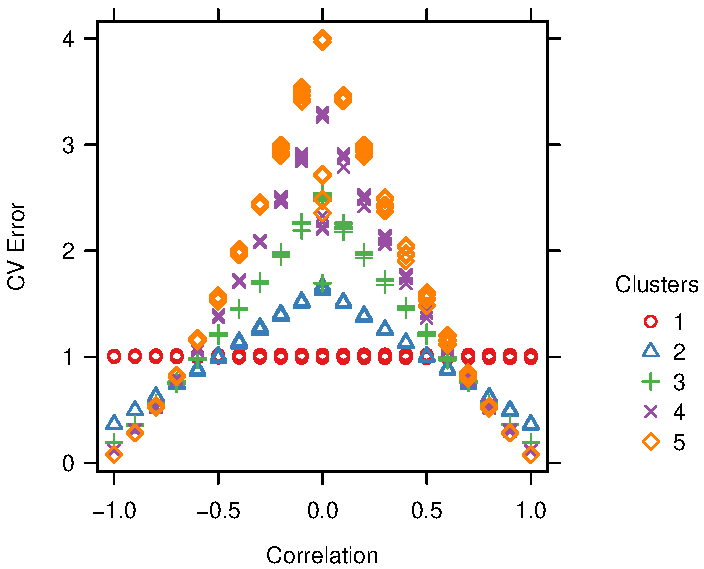
\includegraphics[width=25pc]{demo/nullcorr/equal.pdf}
\caption{Cross-validation error on $10$ replicates, with the number of
clusters $k$ ranging from $1$ to $5$.  Data is generated from two-dimensional
multivariate normal distribution with correlation $\rho$.  The Gabriel
cross-validation criterion chooses the correct answer $k = 1$ whenever
$\rho < 0.5$; the criterion chooses $k = 2$ clusters whenever $|\rho| > 0.5$.}
\label{fig:nullcorr-equal}
\end{figure}


\subsection{Two Clusters}

We will now analyze a simple two-cluster setting, and derive conditions for
Gabriel cross-validation to correctly prefer $k=2$ clusters to $k=1$.

\begin{proposition}
Suppose that $\{(X_i,Y_i)\}_{i=1}^{n+m}$ is data from a single fold of Gabriel
cross-validation, where each $(X,Y)$ pair in $\R^2$ is an independent draw
from an equiprobable mixture of two multivariate normal distributions with
identity covariance. Suppose that the first mixture component has mean $(\muX,
\muY)$, and the second has mean $(-\muX, -\muY)$, where $\muX > 0$ and
$\muY > 0$.  If [Wei, add condition here], then $\CV(2) < \CV(1)$ with
probability tending to one as $m$ and $n$ increase.
\end{proposition}

\begin{proof}
  [Wei, add proof here; you can take most of this from your document,
  ``LDA\_prior\_equal.tex'']
\end{proof}

We confirm the proposition with a simulation.

[Wei, describe simulation here, and include the figure]



\section{Simulation}

In this section, simulation is performed to evaluate the performance of our
proposed methods in locating the ``correct" number of clusters. We compare
with a basket of existing methods including Gap statistics
\citep{tibshirani2001estimating}, Gaussian mixture model-based clustering
\citep{fraley2002model}, CH-index \citep{calinski1974dendrite}, Hartigan
statistics \citep{hartigan1975clustering}, Jump method
\citep{sugar2003finding}, Prediction strength \citep{tibshirani2005cluster},
Bootstrap stability \citep{fang2012selection} in following simulation
settings. We select $L=R$ and $5-$fold cross-validation in row
($m=\frac{4}{5}n$) as default parameter setting for our proposed Gabriel
method. Note that set $L=R$ corresponding to $2-$fold cross-validation in
column.
\begin{enumerate}

  \item Single cluster in $10$ dimensions --- $200$ observations, each
    observation uniformly distributed over $[0,1]$ in each dimension. 

  \item Two clusters in $4$ dimensions --- $50$ i.i.d standard normal
    observations are generated, i.e. generated from multivariate normal
    $\mathcal{N}\left(\boldsymbol\mu,\mathbf{I}\right)$ for each cluster, with
    cluster center $\boldsymbol\mu = (1,0,0,1)$ and $(1,3.5,3.5,1)$
    respectively  

  \item Four clusters in $100$ dimensions ---  Each cluster has $100$ or $150$
    i.i.d standard normal observations, with cluster centers randomly
    generated from multivariate normal distribution
    $\mathcal{N}\left(\mathbf{0},0.65^2\mathbf{I}\right)$

  \item Ten clusters in $100$ dimensions ---  Each cluster has $50$ or $100$
    i.i.d standard normal observations, with cluster centers randomly
    generated from multivariate normal distribution
    $\mathcal{N}\left(\mathbf{0},0.72^2\mathbf{I}\right)$

  \item Four log-normal clusters in $16$ dimensions --- For each cluster, $30$
    or $60$ i.i.d centered log-normal observations are generated from
    $ln\mathcal{N}\left(0,0.5^2 \right)$. The cluster centers are randomly
    generated from multivariate normal distribution
    $\mathcal{N}\left(\mathbf{0},1.2^2\mathbf{I}\right)$

  \item[6.] Three exponential clusters in $20$ dimensions with different
    variance --- $40$ observations in each cluster are generated from centered
    exponential distribution ($exp(\lambda)-1/\lambda$ in each dimension),
    with $\boldsymbol\mu$ randomly generated from
    $\mathcal{N}\left(\mathbf{0},19\mathbf{I}\right)$ and $\lambda = 1, 1/2,
    1/5$ respectively.
\end{enumerate}
Note that in setting 2--6, all clusters are well-separated, i.e. no
overlapping. In fact, any simulated clusters with minimum distance less than
1 unit was discarded, so there is clear definition of true number of
clusters. The parameters in setting 2--6 are chosen such that about half of
the random realization were discarded. The idea is borrowed from
\cite{tibshirani2001estimating}.


Besides the number of clusters selected by each algorithm is returned, we also
give the prediction error (PE) for each algorithm in each setting. The PE is
defined by 
\[
  \PE(k)
    =
      \frac{\|\hat{\mathbf{X}}_k- \boldsymbol{\mu} \|_F}
           {PE_{\text{oracle}}}
\]
where
\[
  \PE_{\text{oracle}} = \min_k \|\hat{\mathbf{X}}_k- \boldsymbol{\mu} \|_F
\]
Matrix $\boldsymbol{\mu}$ consists of true centers of observations in data
matrix $\mathbf{X}$, while $\hat{\mathbf{X}}_k$ is obtained by replacing each
observation in $\mathbf{X}$ by its closest cluster center result from applying
K-means on $\mathbf{X}$ with parameter $k$. Here $k$ is the optimal number of
clusters selected by each algorithm on data $\mathbf{X}$. This is only
possible on simulated data because otherwise one would never know the true
center matrix~$\boldsymbol{\mu}$.


The oracle selected number for each data $\mathbf{X}$ is also given on the
table, which is defined by 
\[
  K_{\text{oracle}}
    =
      \argmin_{k} \|\hat{\mathbf{X}}_k - \boldsymbol{\mu} \|_F
\]

\clearpage

\begin{center}
\footnotesize
\begin{longtable}{lcccccccccccccccc}
\caption{\label{table1} Simulation Results}\\
\toprule
\phantom{Pred.~Strength}
  & \multicolumn{16}{c}{Estimated Number of Clusters} \\
\cmidrule(lr){2-17}
Method
  & 1 & 2 & 3 & 4 & 5 & 6 & 7 & 8 & 9 & 10 & 11 & 12 & 13 & 14 & 15 & NA \\
\midrule
\endfirsthead
\multicolumn{17}{c}%
  {\tablename\ \thetable\ -- \textit{Continued from previous page}} \\
\midrule
\phantom{Pred.~Strength}
  & \multicolumn{16}{c}{Estimated Number of Clusters} \\
\cmidrule(lr){2-17}
Method
  & 1 & 2 & 3 & 4 & 5 & 6 & 7 & 8 & 9 & 10 & 11 & 12 & 13 & 14 & 15 & NA \\
\midrule
\endhead
\multicolumn{17}{r}{\textit{Continued on next page}} \\
\endfoot
\bottomrule
\multicolumn{17}{l}{\footnotesize
  \textsuperscript{$\ast$} CH, Hartigan, and Stability are excluded from
  Setting~1 because they cannot select $k=1$.
}
\endlastfoot
\textit{Setting 1} & \\
Oracle & \textbf{100} & 0 & 0 & 0 & 0 & 0 & 0 & 0 & 0 & 0 & 0 & 0 & 0 & 0 & 0 & 0 & 1 \\
Gap & \textbf{96} & 0 & 0 & 0 & 0 & 0 & 0 & 1 & 0 & 0 & 0 & 0 & 0 & 1 & 2 & 0 & 5.3 $\pm$ 25.4 \\
Gaussian-Mix & \textbf{100} & 0 & 0 & 0 & 0 & 0 & 0 & 0 & 0 & 0 & 0 & 0 & 0 & 0 & 0 & 0 & 1.0 $\pm$ 0.0 \\
CH & \textendash & \textendash & \textendash & \textendash & \textendash & \textendash & \textendash & \textendash & \textendash & \textendash & \textendash & \textendash & \textendash & \textendash & \textendash& \textendash & \textendash \\
Hartigan & \textendash & \textendash & \textendash & \textendash & \textendash & \textendash & \textendash & \textendash & \textendash & \textendash & \textendash & \textendash & \textendash & \textendash & \textendash& \textendash & \textendash \\
Jump & \textbf{0} & 0 & 0 & 0 & 0 & 0 & 0 & 0 & 0 & 0 & 0 & 0 & 4 & 25 & 71 & 0 & 115.6 $\pm$ 47.4 \\
Prediction Strength & \textbf{100} & 0 & 0 & 0 & 0 & 0 & 0 & 0 & 0 & 0 & 0 & 0 & 0 & 0 & 0 & 0 & 1.0 $\pm$ 0.0 \\
Stability & \textendash & \textendash & \textendash & \textendash & \textendash & \textendash & \textendash & \textendash & \textendash & \textendash & \textendash & \textendash & \textendash & \textendash & \textendash& \textendash & \textendash \\
Gabriel CV ($5 \times 2$) & \textbf{100} & 0 & 0 & 0 & 0 & 0 & 0 & 0 & 0 & 0 & 0 & 0 & 0 & 0 & 0 & 0 & 1.0 $\pm$ 0.0 \\
Wold CV & \textbf{100} & 0 & 0 & 0 & 0 & 0 & 0 & 0 & 0 & 0 & 0 & 0 & 0 & 0 & 0 & 0 & 1.0 $\pm$ 0.0 \\

\midrule
\textit{Setting 2} & \\
Oracle & 0 & \textbf{100} & 0 & 0 & 0 & 0 & 0 & 0 & 0 & 0 & 0 & 0 & 0 & 0 & 0 & 0 & 1 \\
Gap & 0 & \textbf{79} & 19 & 0 & 1 & 0 & 0 & 0 & 0 & 0 & 0 & 0 & 0 & 1 & 0 & 0 & 5.1 $\pm$ 11.0 \\
Gaussian-Mix & 0 & \textbf{85} & 1 & 0 & 0 & 0 & 0 & 0 & 0 & 0 & 0 & 0 & 0 & 0 & 0 & 14 & 1.1 $\pm$ 0.8 \\
CH & 0 & \textbf{100} & 0 & 0 & 0 & 0 & 0 & 0 & 0 & 0 & 0 & 0 & 0 & 0 & 0 & 0 & 1.0 $\pm$ 0.0 \\
Hartigan & 0 & \textbf{0} & 40 & 19 & 14 & 7 & 5 & 2 & 6 & 2 & 0 & 1 & 3 & 0 & 1 & 0 & 24.5 $\pm$ 20.5 \\
Jump & 0 & \textbf{0} & 0 & 0 & 0 & 0 & 0 & 0 & 0 & 0 & 0 & 4 & 12 & 21 & 63 & 0 & 47.1 $\pm$ 29.0 \\
Prediction Strength & 0 & \textbf{100} & 0 & 0 & 0 & 0 & 0 & 0 & 0 & 0 & 0 & 0 & 0 & 0 & 0 & 0 & 1.0 $\pm$ 0.0 \\
Stability & 0 & \textbf{100} & 0 & 0 & 0 & 0 & 0 & 0 & 0 & 0 & 0 & 0 & 0 & 0 & 0 & 0 & 1.0 $\pm$ 0.0 \\
Gabriel CV & 0 & \textbf{89} & 11 & 0 & 0 & 0 & 0 & 0 & 0 & 0 & 0 & 0 & 0 & 0 & 0 & 0 & 3.0 $\pm$ 6.6 \\
Gabriel-5X2 CV & 0 & \textbf{92} & 7 & 1 & 0 & 0 & 0 & 0 & 0 & 0 & 0 & 0 & 0 & 0 & 0 & 0 & 2.3 $\pm$ 5.0 \\
Gabriel-proportion CV & 0 & \textbf{88} & 5 & 0 & 1 & 1 & 0 & 1 & 0 & 1 & 1 & 0 & 1 & 0 & 1 & 0 & 5.5 $\pm$ 17.1 \\
Gabriel-proportion-5X2 CV & 0 & \textbf{90} & 1 & 2 & 0 & 1 & 1 & 1 & 0 & 3 & 0 & 1 & 0 & 0 & 0 & 0 & 4.4 $\pm$ 13.4 \\
Wold CV & 0 & \textbf{67} & 21 & 10 & 1 & 1 & 0 & 0 & 0 & 0 & 0 & 0 & 0 & 0 & 0 & 0 & 7.4 $\pm$ 12.5 \\

\midrule
\textit{Setting 3} & \\
Oracle & 0 & 0 & 0 & \textbf{100} & 0 & 0 & 0 & 0 & 0 & 0 & 0 & 0 & 0 & 0 & 0 & 0 & 1 \\
Gap & 0 & 0 & 0 & \textbf{100} & 0 & 0 & 0 & 0 & 0 & 0 & 0 & 0 & 0 & 0 & 0 & 0 & 1.0 $\pm$ 0.0 \\
Gaussian-Mix & 78 & 6 & 2 & \textbf{1} & 4 & 2 & 2 & 0 & 0 & 2 & 0 & 1 & 0 & 0 & 2 & 0 & 33.2 $\pm$ 13.9 \\
CH & 0 & 16 & 24 & \textbf{60} & 0 & 0 & 0 & 0 & 0 & 0 & 0 & 0 & 0 & 0 & 0 & 0 & 7.2 $\pm$ 8.9 \\
Hartigan & 0 & 0 & 9 & \textbf{80} & 8 & 3 & 0 & 0 & 0 & 0 & 0 & 0 & 0 & 0 & 0 & 0 & 2.1 $\pm$ 3.1 \\
Jump & 0 & 0 & 0 & \textbf{0} & 0 & 0 & 0 & 0 & 0 & 0 & 0 & 0 & 0 & 9 & 91 & 0 & 8.6 $\pm$ 0.7 \\
Prediction Strength & 47 & 0 & 0 & \textbf{53} & 0 & 0 & 0 & 0 & 0 & 0 & 0 & 0 & 0 & 0 & 0 & 0 & 20.2 $\pm$ 21.2 \\
Stability & 0 & 0 & 0 & \textbf{35} & 56 & 9 & 0 & 0 & 0 & 0 & 0 & 0 & 0 & 0 & 0 & 0 & 1.7 $\pm$ 0.5 \\
Gabriel CV (Nearest; $2 \times 2$) & 0 & 0 & 0 & \textbf{100} & 0 & 0 & 0 & 0 & 0 & 0 & 0 & 0 & 0 & 0 & 0 & 0 & 1.0 $\pm$ 0.0 \\
Gabriel CV (Nearest; $5 \times 2$) & 0 & 0 & 0 & \textbf{100} & 0 & 0 & 0 & 0 & 0 & 0 & 0 & 0 & 0 & 0 & 0 & 0 & 1.0 $\pm$ 0.0 \\
Gabriel CV (LDA Equal; $2 \times 2$) & 0 & 0 & 0 & \textbf{100} & 0 & 0 & 0 & 0 & 0 & 0 & 0 & 0 & 0 & 0 & 0 & 0 & 1.0 $\pm$ 0.0 \\
Gabriel CV (LDA Equal; $5 \times 2$) & 0 & 0 & 0 & \textbf{100} & 0 & 0 & 0 & 0 & 0 & 0 & 0 & 0 & 0 & 0 & 0 & 0 & 1.0 $\pm$ 0.0 \\
Gabriel (CV LDA Prop.; $2 \times 2$) & 0 & 0 & 0 & \textbf{100} & 0 & 0 & 0 & 0 & 0 & 0 & 0 & 0 & 0 & 0 & 0 & 0 & 1.0 $\pm$ 0.0 \\
Gabriel (CV LDA Prop.; $5 \times 2$) & 0 & 0 & 0 & \textbf{100} & 0 & 0 & 0 & 0 & 0 & 0 & 0 & 0 & 0 & 0 & 0 & 0 & 1.0 $\pm$ 0.0 \\
Wold CV & 0 & 0 & 0 & \textbf{100} & 0 & 0 & 0 & 0 & 0 & 0 & 0 & 0 & 0 & 0 & 0 & 0 & 1.0 $\pm$ 0.0 \\

\midrule
\textit{Setting 4} & \\*
Gap & $\cdot$ & $\cdot$ & $\cdot$ & $\cdot$ & $\cdot$ & $\cdot$ & $\cdot$ & $\cdot$ & $\cdot$ & \textbf{100} & $\cdot$ & $\cdot$ & $\cdot$ & $\cdot$ & $\cdot$ & $\cdot$ \\*
Gaussian-Mix & 44 & 5 & 10 & 9 & 3 & 5 & 5 & 4 & 5 & \textbf{3} & 3 & 2 & 1 & 1 & $\cdot$ & $\cdot$ \\*
CH & $\cdot$ & 38 & 16 & 12 & 7 & 10 & 7 & 4 & 2 & \textbf{4} & $\cdot$ & $\cdot$ & $\cdot$ & $\cdot$ & $\cdot$ & $\cdot$ \\*
Hartigan & $\cdot$ & $\cdot$ & 1 & $\cdot$ & 5 & 8 & 5 & 19 & 19 & \textbf{16} & 13 & 5 & 9 & $\cdot$ & $\cdot$ & $\cdot$ \\*
Jump & $\cdot$ & $\cdot$ & $\cdot$ & $\cdot$ & $\cdot$ & $\cdot$ & $\cdot$ & $\cdot$ & $\cdot$ & \textbf{100} & $\cdot$ & $\cdot$ & $\cdot$ & $\cdot$ & $\cdot$ & $\cdot$ \\*
Pred.~Strength & 100 & $\cdot$ & $\cdot$ & $\cdot$ & $\cdot$ & $\cdot$ & $\cdot$ & $\cdot$ & $\cdot$ & \textbf{0} & $\cdot$ & $\cdot$ & $\cdot$ & $\cdot$ & $\cdot$ & $\cdot$ \\*
Stability & $\cdot$ & $\cdot$ & $\cdot$ & $\cdot$ & $\cdot$ & $\cdot$ & $\cdot$ & $\cdot$ & $\cdot$ & \textbf{0} & 9 & 16 & 37 & 23 & 15 & $\cdot$ \\*
Gabriel CV & $\cdot$ & $\cdot$ & $\cdot$ & $\cdot$ & $\cdot$ & $\cdot$ & $\cdot$ & $\cdot$ & $\cdot$ & \textbf{100} & $\cdot$ & $\cdot$ & $\cdot$ & $\cdot$ & $\cdot$ & $\cdot$ \\*
Gabriel CV (Rot) & $\cdot$ & $\cdot$ & $\cdot$ & $\cdot$ & $\cdot$ & $\cdot$ & $\cdot$ & $\cdot$ & $\cdot$ & \textbf{100} & $\cdot$ & $\cdot$ & $\cdot$ & $\cdot$ & $\cdot$ & $\cdot$ \\*
Wold CV & $\cdot$ & $\cdot$ & $\cdot$ & $\cdot$ & $\cdot$ & $\cdot$ & $\cdot$ & $\cdot$ & $\cdot$ & \textbf{100} & $\cdot$ & $\cdot$ & $\cdot$ & $\cdot$ & $\cdot$ & $\cdot$ \\*

\midrule
\textit{Setting 5} & \\
Oracle & 0 & 0 & 0 & \textbf{100} & 0 & 0 & 0 & 0 & 0 & 0 & 0 & 0 & 0 & 0 & 0 & 0 & 1 \\
Gap & 0 & 0 & 0 & \textbf{100} & 0 & 0 & 0 & 0 & 0 & 0 & 0 & 0 & 0 & 0 & 0 & 0 & 1.0 $\pm$ 0.0 \\
Gaussian-Mix & 0 & 0 & 0 & \textbf{61} & 31 & 7 & 1 & 0 & 0 & 0 & 0 & 0 & 0 & 0 & 0 & 0 & 1.9 $\pm$ 1.3 \\
CH & 0 & 3 & 15 & \textbf{59} & 19 & 4 & 0 & 0 & 0 & 0 & 0 & 0 & 0 & 0 & 0 & 0 & 7.7 $\pm$ 15.5 \\
Hartigan & 0 & 0 & 17 & \textbf{63} & 9 & 4 & 1 & 4 & 1 & 1 & 0 & 0 & 0 & 0 & 0 & 0 & 5.6 $\pm$ 9.0 \\
Jump & 0 & 0 & 0 & \textbf{1} & 0 & 0 & 0 & 0 & 0 & 0 & 0 & 0 & 0 & 28 & 71 & 0 & 12.5 $\pm$ 2.6 \\
Prediction Strength & 76 & 5 & 9 & \textbf{10} & 0 & 0 & 0 & 0 & 0 & 0 & 0 & 0 & 0 & 0 & 0 & 0 & 116.9 $\pm$ 66.9 \\
Stability & 0 & 3 & 1 & \textbf{23} & 44 & 13 & 9 & 2 & 0 & 0 & 0 & 1 & 1 & 2 & 1 & 0 & 5.1 $\pm$ 9.8 \\
Gabriel CV ($5 \times 2$) & 0 & 0 & 0 & \textbf{100} & 0 & 0 & 0 & 0 & 0 & 0 & 0 & 0 & 0 & 0 & 0 & 0 & 1.0 $\pm$ 0.0 \\
Wold CV & 0 & 0 & 1 & \textbf{96} & 3 & 0 & 0 & 0 & 0 & 0 & 0 & 0 & 0 & 0 & 0 & 0 & 1.3 $\pm$ 2.6 \\

\midrule
\textit{Setting 6} & \\
Oracle & 0 & 0 & \textbf{100} & 0 & 0 & 0 & 0 & 0 & 0 & 0 & 0 & 0 & 0 & 0 & 0 & 0 & 1 \\
Gap & 0 & 0 & \textbf{0} & 0 & 0 & 0 & 0 & 0 & 1 & 1 & 4 & 7 & 11 & 34 & 42 & 0 & 18.5 $\pm$ 7.3 \\
Gaussian-Mix & 0 & 0 & \textbf{84} & 15 & 0 & 0 & 0 & 0 & 0 & 0 & 0 & 0 & 0 & 0 & 0 & 1 & 1.5 $\pm$ 1.3 \\
CH & 0 & 13 & \textbf{73} & 13 & 1 & 0 & 0 & 0 & 0 & 0 & 0 & 0 & 0 & 0 & 0 & 0 & 3.8 $\pm$ 7.0 \\
Hartigan & 0 & 0 & \textbf{91} & 5 & 2 & 0 & 1 & 0 & 1 & 0 & 0 & 0 & 0 & 0 & 0 & 0 & 1.6 $\pm$ 2.3 \\
Jump & 0 & 0 & \textbf{0} & 0 & 0 & 0 & 0 & 0 & 0 & 0 & 0 & 4 & 11 & 40 & 45 & 0 & 18.8 $\pm$ 7.4 \\
Prediction Strength & 14 & 0 & \textbf{86} & 0 & 0 & 0 & 0 & 0 & 0 & 0 & 0 & 0 & 0 & 0 & 0 & 0 & 6.8 $\pm$ 16.4 \\
Stability & 0 & 0 & \textbf{18} & 44 & 29 & 6 & 0 & 0 & 0 & 0 & 0 & 0 & 0 & 0 & 0 & 3 & 5.0 $\pm$ 3.2 \\
Gabriel CV (Nearest; $2 \times 2$) & 0 & 4 & \textbf{89} & 7 & 0 & 0 & 0 & 0 & 0 & 0 & 0 & 0 & 0 & 0 & 0 & 0 & 1.5 $\pm$ 1.9 \\
Gabriel CV (Nearest; $5 \times 2$) & 0 & 0 & \textbf{99} & 1 & 0 & 0 & 0 & 0 & 0 & 0 & 0 & 0 & 0 & 0 & 0 & 0 & 1.0 $\pm$ 0.4 \\
Gabriel CV (LDA Equal; $2 \times 2$) & 0 & 4 & \textbf{95} & 1 & 0 & 0 & 0 & 0 & 0 & 0 & 0 & 0 & 0 & 0 & 0 & 0 & 1.5 $\pm$ 3.0 \\
Gabriel CV (LDA Equal; $5 \times 2$) & 0 & 1 & \textbf{97} & 2 & 0 & 0 & 0 & 0 & 0 & 0 & 0 & 0 & 0 & 0 & 0 & 0 & 1.2 $\pm$ 1.0 \\
Gabriel (CV LDA Prop.; $2 \times 2$) & 0 & 3 & \textbf{96} & 1 & 0 & 0 & 0 & 0 & 0 & 0 & 0 & 0 & 0 & 0 & 0 & 0 & 1.4 $\pm$ 2.9 \\
Gabriel (CV LDA Prop.; $5 \times 2$) & 0 & 0 & \textbf{100} & 0 & 0 & 0 & 0 & 0 & 0 & 0 & 0 & 0 & 0 & 0 & 0 & 0 & 1.0 $\pm$ 0.0 \\
Wold CV & 0 & 0 & \textbf{90} & 8 & 2 & 0 & 0 & 0 & 0 & 0 & 0 & 0 & 0 & 0 & 0 & 0 & 1.4 $\pm$ 1.6 \\

\end{longtable}
\end{center}



\noindent
All methods are used with their default parameter setting except for Gap
statistics. We selected the $k$  corresponds to the global maximum of gap
statistics, rather than the default method which selects the smallest $k$ such
that the gap statistics is not more than 1 standard error away from the first
local maximum. This is because among all the possible options, the global
maximum criteria gives the best result in our simulation settings.


The ``\textendash'' sign in Setting~1 is because for CH-index, Hartigen and
Bootstrap stability, the minimum $k$ they can pick is $2$. So they are not
included for comparison since the true $k=1$. Setting $2-4$ have Gaussian
distribution, where the Gaussian mixture model-based clustering suppose to
perform the best. It is only the case for setting $2$. In setting $3$ and $4$,
it has a very poor performance even if the underlying distribution is indeed
Gaussian mixture model. It highlights the difficulties that high dimension
data could cause. Other methods (Gap statistics, CH-index, Hartigan, Jump
method, Prediction strength and Boostrap stability) also have problems in
these two high-dimension settings as we could not find any one with reasonable
performance in terms of finding the correct $k$ in both cases. In terms of PE,
Boostrap stability and Gap statistics have reasonable performance, but come
with the price of picking larger $k$. Our proposed Gabriel method (also Wold
CV method) clearly stands out from the basket of existing methods using either
measure under the high-dimension setting $3$ and $4$.


Setting $5$ and $6$ corresponding to the situation where data are heavy-tailed
instead of normal distributed, coupled with unequal number of observations or
unequal variance for different clusters. From Table \ref{table1}, we can see
that our proposed Gabriel method is robust and has superior performance
compare with other methods. Because one can hardly tell the underlying
distribution of data in practice, the resilience to non-Gaussian data gives
the Gabriel method a clear edge. 



\section{Real data application}

We also applied our proposed method to three real world data sets obtained
from the University of California Irvine machine learning repository. The
first and third data sets are selected because there are clear number of
clusters in those two data sets. The second data set is used as a benchmark
data set since it was widely used in literature.


The first one is congress voting data which consists of voting records of
$98$th United States Congress, $2$nd session. This data set includes votes for
each of the U.S. House of Representatives Congressmen on the $16$ key votes
identified by the \textit{CQA} (Congressional Quarterly Almanac). For each
vote, each Congressman either vote positively ``yea" (voted for/paired
for/announced for),  negatively ``nay'' (voted against/paired
against/announced against) or position unknown ``?". We took out those records
contain ``?" before comparing each algorithm. It results in $232$ remaining
records, with $124$ democrat and $108$ republican. 


The second data set is the well-known Wisconsin breast cancer data set \citep{mangasarian1990pattern}. After excluding the records with missing data, this data set consists records of $683$ patients, each with measurements of nine attributes of their biopsy specimens. It is known that there exist at least two groups of patients: $444$ patients with benign specimens and $239$ patients with malignant specimens.\\

The third data set is the Sonar data returned from two targets -- a metal
cylinder and a rock with similar shape, which is first studied by
\cite{gorman1988analysis} using a neural network. Both targets were impinged
by pulse which was a wide-band linear FM chirp $(ka = 55.6)$. Returns were
collected at a range of $10$ meters and obtained from the cylinder at aspect
angles spanning $90^{\circ}$ and from the rock at aspect angles spanning
$180^{\circ}$. The data set contains $208$ returns ($111$ cylinder returns and
$97$ rock returns), with each composed of $60$ spectral samples, normalized to
take on values between $0$ and $1$. So the data has $60$ features with clearly
$2$ clusters. 


\begin{table}[H]
\begin{center}
\caption{\label{table2} Number of clusters selected by each algorithm}
\begin{tabular}{lccccc}
    \hline                  
 & Congress Voting && Breast Cancer && Sonar \\ \hline                    
CH-index & $2$ && $2$  && $2$    \\
Hartigan & $3$ && $3$  &&  $3$   \\
Jump & $9$ && $9$ && $10$  \\   
Prediction strength & $2$ &&  $2$ && $1$    \\
Bootstrap stability & $2$ &&  $2$ &&  $10$   \\ 
Gap & $10$ && $9$ && $10$  \\   
Gaussian-Mix & $7$ && $5$ && $1$  \\   
Gabriel & $2$  && $3$  && $2$  \\    
Wold & $2$ && $3$ && $10$ \\  \hline 
\end{tabular}
\end{center}
\hspace{0.5in} \footnotesize {All the algorithms executed with their default parameter settings with $k$ ranges from $1$ to $10$}
\end{table} 

Since most congressmen vote base on their parties' interest, $2$ parties
(Democratic and Republican) represent two clusters in this data set. So the
optimal number should be two. Close inspection shows \textit{kmeans} with
$k=2$ separates the two parties very well with the lowest miss-classification
error $10.43\%$ ($k=3$ has $14.78\%$). Note that CH-index and Bootstrap
stability also return $k=2$, but $2$ is the lower bound those methods can
select for $k$. So it's not clear they actually choose $k=2$ or they hit the
lower bound (they would pick $k=1$ if allowed). For the breast cancer data,
it's know to have at least $2$ cluster based on whether it's benign specimens
or not. But it doesn't mean the optimal $k$ should be $2$.
\cite{fujita2014non} noticed that the malign group is quite heterogeneous and
can be further clustered into at least two subgroups. Hence, the result $k=3$
given by our proposed Gabriel method (as well as Wold method) make sense. For
the Sonar data set which is relatively high-dimension, only our proposed
Gabriel method and CH-index selects $k=2$. Majority of the methods collapse to
either select the maximum or select the minimum number, underline how
difficult it was to pick the right $k$ when dimension increases. 


\section{Conclusion}

In this paper, we proposed a novel approach to estimate the number of
clusters. The intuition behind our proposed methods is to transfer the
unsupervised learning problem into supervised learning problem via novel form
of cross validation. We proved the self-consistency for our proposed Gabriel
CV method as well as its asymptotic property with noise, and showed the
robustness of our method by simulation. Our method has very good performance
in our limited simulation settings, and clearly the superior one when data is
high dimension or is heavy-tailed.


\section*{\textbf{APPENDIX}}
\appendix
\section{Wold CV estimation} \label{app:foobar}
\begin{itemize}
	\item For each $k = 1,2,...,k_{max}$
	\begin{enumerate}
		\item Randomly draw some entries in $\mathbf{X}$ missing, keep those hold-out values in vector $V_{true}$
		\item Impute the missing values with column mean or $0$, denote the imputed data as $\mathbf{X}_{new}$
		\item Apply the iterative procedure below until converge or stopping criteria reached
		\begin{itemize}
			\item Apply $K$-mean on data set $\mathbf{X}_{new}$ with parameter $k$
			\item Substitute each observation in $\mathbf{X}_{new}$ by its nearest center, get new data $\mathbf{X}^c_{new}$ ($\mathbf{X}_{new}$ keep the same)
			\item Replace (impute) those imputed values in $\mathbf{X}_{new}$ with the corresponding entries in $\mathbf{X}^c_{new}$
			\item Calculate the difference between the old and newly imputed values, check whether or not they coincide (converge) 
		\end{itemize}
		\item Obtain the last imputed entry values of converged $\mathbf{X}_{new}$, denote it by $V_{converge}$
		\item Calculate the prediction error  $Error_k = ||V_{true} - V_{converge}||^2$ 
	\end{enumerate}
	\item For each CV folder, repeat above procedure and obtain the $Error_k$ for each $k$
	\item Average $Error_k$ across all folders for each $k$, and then select the $k$ corresponding to the minimum average $Error_k$ 
\end{itemize}


\section{Technical Lemmas}
\label{app:technical-lemmas}

\begin{lemma}\label{lem:truncated-normal-moments}

If $Z$ is a standard normal random variable, then
\[
  \E(Z \mid a < Z < b)
    = - \frac{\varphi(b) - \varphi(a)}
             {\Phi(b) - \Phi(a)}
\]
and
\[
  \E\{(Z - \delta)^2 \mid a < Z < b\}
    = \delta^2 + 1
    - \frac{  (b - 2 \delta) \varphi(b)
            - (a - 2 \delta) \varphi(a)}
           {\Phi(b) - \Phi(a)}
\]
for all constants $a$, $b$, and $\delta$, where $\varphi(z)$ and $\Phi(z)$ are
the standard normal probability density and cumulative distribution functions.
These expressions are valid for $a = -\infty$ or $b = \infty$ by taking
limits.

\end{lemma}
\begin{proof}
We will derive the expression for the second moment.  Integrate to get
\begin{align*}
  \E[ (Z - \delta)^2 1\{Z < b\}]
    &= \int_{-\infty}^b (z - \delta)^2 \varphi(z) \, dz \\
    &= (\delta^2 + 1) \Phi(b) - (b - 2 \delta) \varphi(b).
\end{align*}
Now,
\[
  \E\{(Z - \delta)^2 \mid a < Z < b\}
    =
    \frac{  \E[ (Z - \delta)^2 1\{Z < b\}]
          - \E[ (Z - \delta)^2 1\{Z < a\}]}
         { \Phi(b) - \Phi(a) }.
\]
\end{proof}

Lemma~\ref{lem:truncated-normal-moments} has some important special cases:
\begin{align*}
  \E\{Z \mid Z > 0\} &= 2 \varphi(0) = \sqrt{2 / \pi}, \\
  \E\{(Z - \delta)^2 \mid Z > 0 \}
    &= \delta^2 + 1 - 4 \delta \varphi(0), \\
  \E\{(Z - \delta)^2 \mid Z < 0 \}
    &= \delta^2 + 1 + 4 \delta \varphi(0).
\end{align*}



\bibliography{references}
\bibliographystyle{apalike}
\end{document}
